\documentclass{artikel1}
\usepackage[resetfonts]{cmap}
\usepackage{lmodern}
\usepackage[slovak]{babel}
\usepackage[utf8]{inputenc}
\usepackage[T1]{fontenc}
\usepackage{graphicx}
\usepackage{pdfpages}
\usepackage{microtype}

\usepackage[backend=biber,
            style=alphabetic,
            maxnames=5,
            alldates=iso,
            seconds=true]{biblatex}
\addbibresource{databaze-literatury.bib}

\usepackage[xindy]{imakeidx}
\makeindex[options=-L slovak-large -C utf8]
\usepackage{hyperref} %xindy and hyperref really don't want to play together
    
\title{Problém anonymity a~cenzúry na internete}
\author{Adam Renčo}
\date{December 2022}

\begin{document}
\setcounter{page}{5} % označíme CV ako 5. stranu, aby hyperref fungoval správne pri odkazovaní sa na 1. stranu
\includepdf{cv.pdf} %vytvorené z cv.tex
\setcounter{page}{1}
\maketitle

\section{Úvod}

Rýchly pokrok doby \index{doby@doba} vyvoláva výrazné zvyšovanie percenta ľudskej interakcie vykonávanej pomocou technologických zariadení (internetu) \index{internet} na úkor osobných interakcií. Jedným z~dôvodov, prečo ľudia preferujú používanie internetu, je možnosť \index{anonymity@anonymita} anonymity. Tá však prináša aj mnohé nevýhody, pretože dáva niektorým ľuďom pocit, že nemusia dodržiavať pravidlá spoločnosti. Prílišné obmedzenia anonymity ale naopak často narúšajú slobodu prejavu a~prinášajú cenzurovanie názorov.\\\\
Je veľmi dôležité nájsť správnu hranicu medzi absolútnou voľnosťou a~limitovaním možností konania na internete. Je potrebné chrániť užívateľov pred možnými útokmi, zamedzovať šírenie dezinformácií a~zabraňovať rôznym iným zneužitiam internetu. Zároveň je ale nutné nenarušovať súkromie a~neobmedzovať voľnú ľudskú interakciu.\\\\

\begin{figure}[htbp]
    \begin{center}
        \includegraphics[width=0.85\textwidth]{censor}
    \end{center}
    \caption{Bitmapová ilustrácia cenzúry}
    \label{censor}
\end{figure}

\section{Drastické riešenia v~iných krajinách}

Vlády všetkých štátov sa už musia zaoberať riešením problémov súvisiacich s~anonymitou na internete. Jedným z~riešení je anonymitu zredukovať alebo úplne odstrániť. Toto riešenie však nie je ideálne, pretože prekračuje niektoré morálne a~právne hranice\index{hranice!morálne}\index{hranice!právne}.

\subsection{Južná Kórea}

V~Južnej Kórei \index{Kórea!južná} vláda reagovala na nárast spáchaných samovrážd viazaných na kyberšikanu zavedením povinnosti zadania Resident Registration Number (podobné ako naše rodné číslo) na umožnenie používania niektorých webových stránok. Vládne nariadenie malo znížiť počet nepravdivých novinárskych správ a~zabrániť šikane pomocou jednoduchšieho rozpoznania identity tvorcu správ. Nariadenie malo však aj zlé následky. Potlačilo slobodu prejavu a~boli ním potláčané prejavy kritizujúce vládu.~\cite{, south-korea-cfc}

\subsection{Čína}

V~Číne \index{Čína} je taktiež požadované overenie identity podľa identifikačného čísla človeka pre možnosť plného využívania internetu. Cenzúra \index{cenzúra} je tu ale oveľa prísnejšia a~štát má skoro úplnú kontrolu nad novinárskymi článkami. Zároveň sú často blokované publikácie materiálov nevyhovujúcich vláde. Informácie a~stránky, ku ktorým sa užívatelia vedia dostať, sú filtrované. Kontroverzné udalosti sú častokrát utajované a~skrývané pred verejnosťou. Od roku 2021 platí nariadenie pre deti pod 18 rokov, ktoré ich obmedzuje na 3 hodiny hrania online počítačových hier týždenne, teda od 20. do 21. hodiny v~piatok a~cez víkend. Kvôli tomuto nariadeniu sa niektorí tínedžeri pokúšajú o~získanie identifikačných údajov osôb starších ako 18 rokov.~\cite{wiki-china, china-game-limit}

\subsection{Severná Kórea}

Severná Kórea \index{Kórea!severná} má nariadenia ešte prísnejšie. Väčšinová časť populácie nemá umožnený prístup k~vonkajšiemu internetu, prístup majú iba k~sieti od domáceho prevádzkovateľa Kwangmyong, ktorý je \index{monitorovanie} monitorovaný severokórejskou vládou. Informácie, ktoré sa k~verejnosti dostávajú sú tak limitované a~upravené podľa potreby vlády.  K~vonkajšiemu internetu \index{internet} má prístup iba pár inštitúcií a~veľmi malá elita. Spojenie je ale stále kontrolované.~\cite{wiki-nk-i, wiki-nk-c}

\section{Nutnosť ideálneho riešenia}

Je zrejmé, že ani jeden z~extrémov \index{extrém} medzi plnou a~žiadnou anonymitou nie je ideálnym riešením. Zavedenie hociktorého z~nich síce prináša svoje výhody, ale zároveň sú oba nemorálne a~porušujú ľudské práva. Preto je veľmi nutné dôkladne zvážiť všetky faktory ovplyvňujúce časti internetu, a~pre každú z~nich upraviť nariadenia pre anonymitu tak, aby vyhovovali ako právnym, tak aj morálnym stanoviskám.\\\\
Nútená identifikácia by mohla veľmi pomôcť na sociálnych sietiach. Zvýšila by sa tak bezpečnosť a~správanie užívateľov by tak mohlo byť oveľa lepšie regulované. Takáto forma \index{bezpečnosť} bezpečnosti by bola zväčša najdôležitejšia pre ochranu maloletých a~pomohla by zamedziť „Catfishingu“. Ľudia by mali istotu, že komunikujú s~overeným človekom \index{človek} a~nie s~podvodníkom, \index{podvodník} ktorý sa ich snaží oklamať.\\\\
Zároveň je ale nutné nezrušiť miesta na internete, kde si človek môže zachovať svoju anonymitu. Existujú stránky, kde sa ľudia, ktorí si nevedia poradiť so svojimi problémami, môžu zveriť s~tým, čo ich trápi, a~vypýtať si pochopenie alebo rady ako pokračovať. V~takýchto prípadoch je u veľmi dôležité zachovanie anonymity, pretože je jednoduchšie sa zveriť niekomu, s~kým človek nemá žiadne spojenie, a~tým pádom sa k~nemu nedostanú žiadne nežiadúce následky. Zachovanie anonymity je dôležité aj z~pohľadu možnosti voľnej diskusie tabu tém a~názorov nevyhovujúcich vláde alebo iným mocenským orgánom.

\section{Záver}
S~veľkým nárastom pomeru ľudských interakcií na internetových \index{internet} sietiach je veľmi dôležité vybrať správne riešenia na všetky časti tohto problému, pretože budú mať silný dopad na celú spoločnosť. Preto je nevyhnutné preskúmať všetky možnosti a~faktory pri tvorení a~ustanovení nariadení.\\\\

\begin{figure}[htbp]
    \begin{center}
        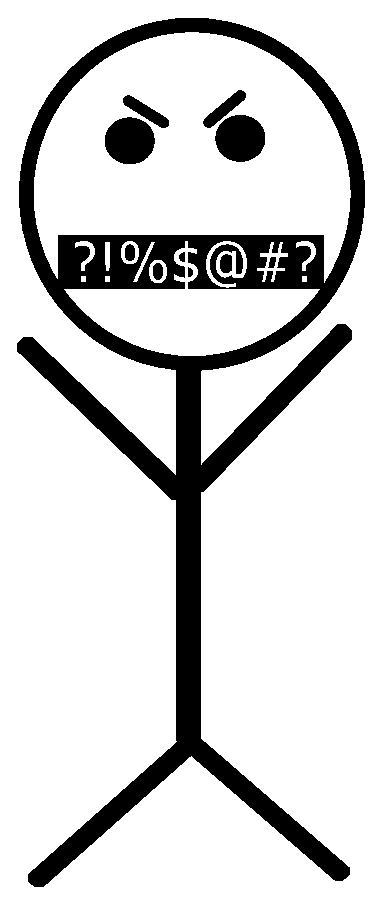
\includegraphics[width=0.30\textwidth]{censored-person.eps}
    \end{center}
    \caption{Vektorová ilustrácia cenzúry}
    \label{censored-nospeaking}
\end{figure}

\printbibliography[heading=bibintoc]
\begingroup
\let\clearpage\relax
\printindex
\endgroup
\end{document}
